\documentclass[11pt]{article}
\usepackage[margin = 1in, paperwidth = 8.5in, paperheight = 11in]{geometry}
\usepackage{amsfonts}
\usepackage{graphicx}


\def\eq1{y = \frac{x}{3x^2+x+1}}

\def\labelaxis{Remember to include a scale and label your axis}

\begin{document}

\tableofcontents

\title{My Practice \LaTeX \ Document}
\author{Ajay Kumar}
\date{\today}
\maketitle

This is my first LaTeX document.\\
Suppose I want to build a rectangle with sides
$(x+1)$ and $(x+3)$, then the area of rectangle is given by: $A = x^2+4x+3$

This is my first LaTeX document.


Suppose I want to build a rectangle with sides
$(x+1)$ and $(x+3)$, then the area of rectangle is given by: $A = x^2+4x+3$

Suppose I want to build a rectangle with sides
$(x+1)$ and $(x+3)$, then the area of rectangle is given by: $$A = x^2+4x+3$$

superscripts: $2x^3$

superscripts: $$2x^3$$
$$2x^34$$
$$2x^{34}$$
$$2x^{3x+4}$$
$$2x^{3x^4+5}$$

subscripts: $$x_1$$
$$x_{12}$$
$${{x_1}_2}_3$$

Greek Letters:
$$\pi$$
$$\alpha$$
$$A = \pi r^2$$

Trig:
$$y = \sin{x}$$
$$y = \cos{x}$$
$$y = \tan{x}$$

Log:
$$\log{x}$$
$$\ln{x}$$
$$\log_5{x}$$

square roots:
$$\sqrt{2}$$
$$\sqrt[3]{2}$$
$$\sqrt[3]{x^2+y^2}$$
$$\sqrt{1+\sqrt{x}}$$

fractions:

About 2/3 of the glass is full.

About $2/3$ of the glass is full. Nothing changes here.

About $\frac{2}{3}$ of the glass is full.

About $\displaystyle{\frac{2}{3}}$ of the glass is full.

$$\frac{x}{x^2+x+1}$$

$$\frac{\sqrt{x+1}}{\sqrt{x-1}}$$

$$\frac{1}{1+\frac{1}{x}}$$

$$\frac{1}{1+\displaystyle{\frac{1}{x}}}$$

$$\sqrt{\frac{x}{x^2+x+1}}$$

Brackets, Tabels and Arrays
$$(x+1)$$

$$3[2+(x+1)]$$

${a,b,c}$ here we cannot see the breacket

$$\{a,b,c\}$$

$$\$12.55$$

$$3(\frac{2}{5})$$

$$3\left(\frac{2}{5}\right)$$

$$3\left[\frac{2}{5}\right]$$

$$3\left\{\frac{2}{5}\right\}$$

$$|x|$$

$$|\frac{x}{x+1}|$$

$$\left| \frac{x}{x+1} \right|$$

$$\left\{ x^2 \right\}$$

$$\left\{ x^2 \right.$$

$$\left| \frac{dy}{dx} \right|_{x = 1}$$

$$\left. \frac{dy}{dx} \right|_{x = 1}$$

Table:

\begin{tabular}{cccccc}

$x$ & 1 & 2 & 3 & 4 & 5 \\
$f(x)$ & 10 & 11 & 12 & 13 & 14

\end{tabular}


\begin{tabular}{|c|c|c|c|c|c|}
\hline
$x$ & 1 & 2 & 3 & 4 & 5 \\ \hline
$f(x)$ & 10 & 11 & 12 & 13 & 14 \\ \hline

\end{tabular}

Array: eqnarray automatically takes us in to math mode

\begin{eqnarray}
5x^2-9 &=& x+3 \\ 
4x^2 &=& 12 \\ 
x^2 &=& 3 \\ 
x &\approx \pm& 1.732
\end{eqnarray}

No equation numbers:

\begin{eqnarray*}
5x^2-9 &=& x+3 \\ 
4x^2 &=& 12 \\ 
x^2 &=& 3 \\ 
x &\approx& \pm 1.732
\end{eqnarray*}

Lists:

\begin{enumerate}
\item calculator
\item ruler
\item notebook
	\begin{enumerate}
	\item assessments
		\begin{enumerate}
		\item tests
		\item quizes
		\end{enumerate}
	\item home work
	\item notes
	\end{enumerate}
\item graph paper
\item paper
\end{enumerate}

\begin{itemize}
\item calculator
\item ruler
\item notebook
	\begin{itemize}
	\item assessments
		\begin{itemize}
		\item tests
		\item quizes
		\end{itemize}
	\item home work
	\item notes
	\end{itemize}
\item graph paper
\item paper
\end{itemize}

\begin{enumerate}
\item[Commutative] $a+b = b+a$
\item[Associative] $a+(b+c) = (a+b)+c$
\item[Distributive] $a(b+c) = ab + ac$
\end{enumerate}

Text Formatting:

This will produce \textit{italicized} text.

this will produce \textbf{boldfaced} text.

This will produce \textsc{small caps} text.

this will produce \texttt{type writer} text.

Please excuse my dear aunt Sally

Please excuse my \begin{large}
dear aunt Sally
\end{large}

please excuse me \begin{Large}
dear aunt Sally
\end{Large}

please excuse me \begin{huge}
dear aunt Sally
\end{huge}

please excuse me \begin{Huge}
dear aunt Sally
\end{Huge}

please excuse me \begin{small}
dear aunt Sally
\end{small}

please excuse me \begin{tiny}
dear aunt Sally
\end{tiny}

Justification : 

\begin{center}
This is centered Text.
\end{center}

\begin{flushleft}
This is Left Text.
\end{flushleft}

\begin{flushright}
This is Right Text.
\end{flushright}

Sections and Sub Sections:

\section{Linear Functions}
	\subsection{Slope Interccept Form}
	The slope intercept form of the linear function is given by $y = ax+b$.
	\subsection{Standeard Form}
	\subsection{Point Slope Form}
\section{Quadratic Functions}
	\subsection{Vertex Form}
	\subsection{Standard Form}
	\subsection{Factored Form}
	
Making sections and subsections help us to make the table of cotents easy. for this go to top before title and add "\\tableofcontents".

The set of natural numbers is denoted by $\mathbb{N}$.

The set of Integers numbers is denoted by $\mathbb{Z}$.

The set of Real numbers is denoted by $\mathbb{R}$.

Here we use package amsfonts.

Macros:
Macros are used to define our own LaTeX commands, particularly which needs to be typed multiple times.

Graph $\eq1$.

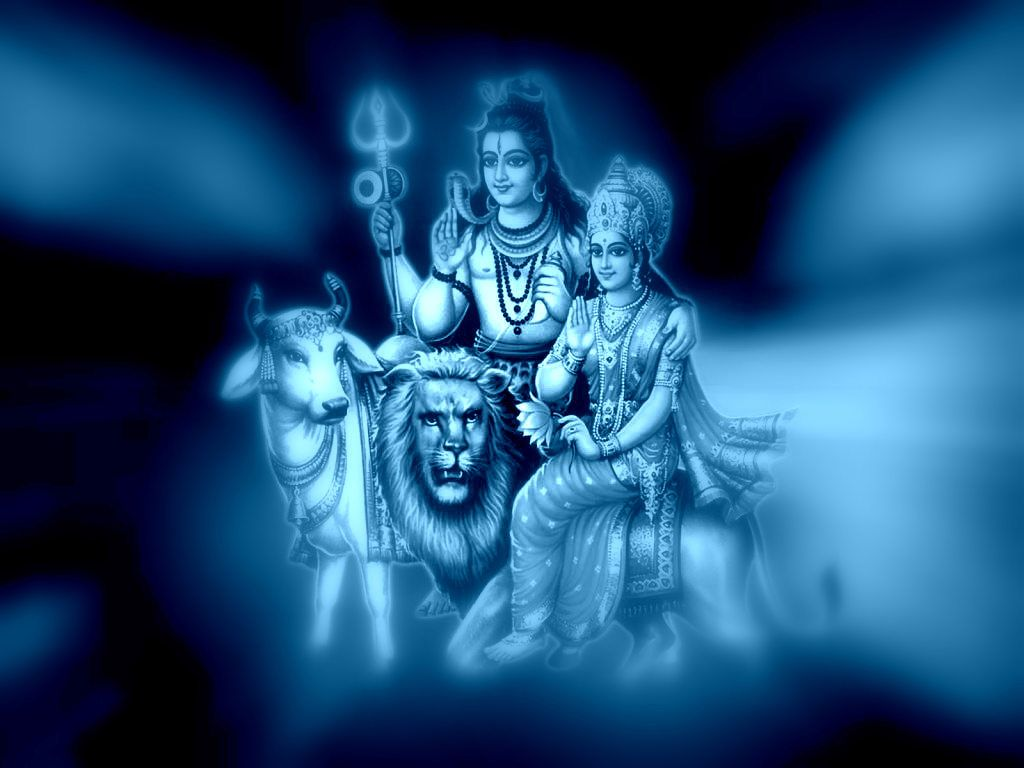
\includegraphics[width = 5in]{last.jpg}

\begin{center}
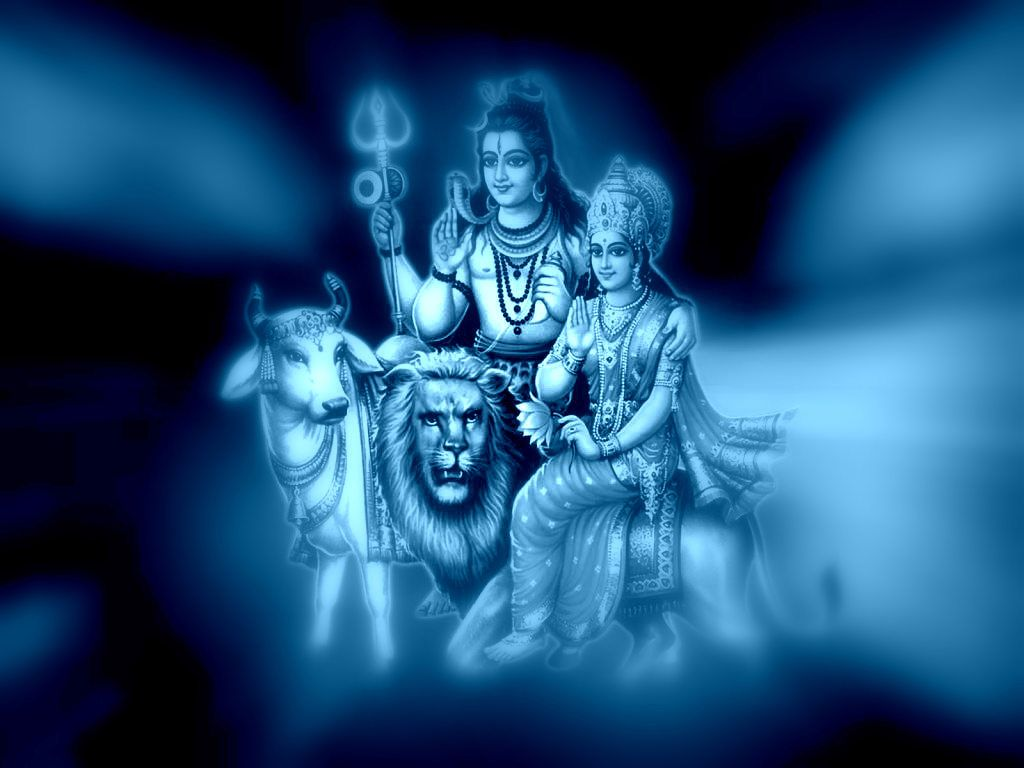
\includegraphics[scale = 0.25, angle = 45]{last.jpg}

We can only use .jpg, .png, .gif and .pdf
\end{center}

Identify the assymptotes for the graph of $\eq1$.

\labelaxis

Comment:

This is comment below


% this is a comment


Calculus Notations:

the function $f(x) = (x-3)^2+\frac{1}{2}$ has domain $\mathrm{D}_f:(-\infty, +\infty)$ and range $\mathrm{R}_f:\left[\frac{1}{2},\infty\right)$. \\

Limit:
$\lim _{x \to a}$

$\lim \limits_{x \to a^+}f(x)$ % from right +, from left -

$\lim \limits_{x \to a}\frac{f(x)-f(a)}{x-a} = f'(a)$

$\displaystyle{\lim \limits_{x \to a}\frac{f(x)-f(a)}{x-a} = f'(a)}$ \\

Integral : 

$\displaystyle{\int \sin x \, dx = - \cos x + C}$

$\displaystyle{\int_a^b}$\\

$\displaystyle{\int \limits_a^b}$

$\displaystyle{\int \limits_2a^b}$

$\displaystyle{\int \limits_{2a}^{b}x^2 \, dx = \left[\frac{x^3}{3}\right]_{2a}^{b}  = \frac{b^3}{3}-\frac{(2a)^3}{3}}$ \\

$\displaystyle{\sum\limits_{n = 1}^{\infty}ar^n = a+ar+ar^2+...+ar^n}$

$\displaystyle{\sum\limits_{n = 1}^{\infty}ar^n = a+ar+ar^2+ \cdots +ar^n}$

$\displaystyle{\int_a^b f(x) \, dx =  \lim \limits_{x \to \infty} \sum \limits_{k = 1}^n f(x_k) \cdot \delta x}$


$\displaystyle{\int_a^b f(x) \, dx =  \lim \limits_{x \to \infty} \sum \limits_{k = 1}^n f(x_k) \cdot \Delta x}$ \\

Vectors:

$\vec{V} = v_1 \vec{i} + v_2 \vec{j} = \langle v_1, v_2 \rangle$


\end{document}